Before we can dive into the mathematics of finance, we first need to review percentages, since we'll find that they are used to express concepts like interests rates.  Once we've gotten comfortable with percentages, we will use them for simple applications like sales tax calculations.

\subsection{Percents}
\marginnote{\textbf{Percent:} \\ number of hundredths}
A percentage is simply another way to represent a fraction or a decimal.  The word ``percent'' means ``per 100,'' or ``number of hundredths.''
\vspace{0.5in}

\begin{proc}{Percents, Fractions, and Decimals}
Since percent (\%) means ``number of hundredths,'' we can convert decimals to percents by multiplying by 100 (or moving the decimal point two places to the right).

We can convert fractions to percents the same way by first writing them as decimals.
\end{proc}
\vspace{0.5in}

\begin{example}[https://www.youtube.com/watch?v=UZHLvEmFrOk]{Converting to Percentages}
Convert each of the following to a percentage:\\

\begin{tabular}{l l l}
(a) $\dfrac{1}{4}$ & (b) $0.02$ & (c) $\dfrac{8}{3}$
\end{tabular}

\begin{center}
\marginnote{\bfseries Solution}
\begin{tabular}{l l l}
(a) $\dfrac{1}{4} = 0.25 = 25\%$ & (b) $0.02 = 2\%$ & (c) $\dfrac{8}{3} = 2.67 = 267\%$
\end{tabular}
\end{center}
\end{example}

\begin{try}[http://izzomath.com/103text/finance/example1.1/story.html]
Convert each of the following to a percentage:\\

\begin{tabular}{l l l}
(a) $\dfrac{3}{5}$ & (b) $0.7$ & (c) 2
\end{tabular}
\end{try}
\vspace{0.25in}

This process can be reversed to convert a percentage to a decimal.

To do so, simply remove the percent symbol and divide the percentage by 100 (i.e. move the decimal point two places to the left).
%\vfill
%\pagebreak

\begin{example}[https://www.youtube.com/watch?v=d770dB9RHIc]{Converting Percents to Decimals}
Convert the following percentages to decimals:\\

\begin{tabular}{l l l}
(a) 17\% & (b) 122\% & (c) 0.15\%
\end{tabular}

\begin{center}
\marginnote{\bfseries Solution}
\begin{tabular}{l l l}
(a) $17\% = 0.17$ & (b) $122\% = 1.22$ & (c) $0.15\% = 0.0015$
\end{tabular}
\end{center}
\end{example}
\vfill
\pagebreak

\subsection{Applied Percent Problems}
Of course, the real goal is to apply what we know about using percentages to applied problems.  These all boil down the statement ``A is P percent of B,'' written \[A = PB.\]  Remember, when translating a sentence into a mathematical expression, ``of'' gets replaced with multiplication.  Each of these applied percentage problems will give two of these pieces and leave the third unknown; our job will be to solve for the third piece.

\begin{example}[https://www.youtube.com/watch?v=8VSRt2PMqJI]{Coffee Survey}
The Frederick News Post did a poll of 1500 people, asking them the following question: ``Do you go to Starbucks at least 3 times a week?'' Of those 1500 polled, 58\% said ``yes.''  How many people replied yes to the survey?\\

\marginnote{\bfseries Solution}
Remember that the keyword ``of'' in a word problem usually refers to multiplication, so ``58\% \textbf{of} 1500'' translates to ``58\% $\cdot$ 1500,'' but to do the multiplication, we need to write the percentage as a decimal:
\[58\% \cdot 1500 = 0.58 \cdot 1500 = 870\]

Thus, 870 people responded ``yes'' to the survey.
\end{example}

\begin{try}[http://izzomath.com/103text/finance/example1.4/story.html]
If there are 6,233 students enrolled this semester, and 59\% of those are women, how many women are attending the college this semester?
\end{try}

From the equation $A=PB$ we can solve for the percentage $P$ by dividing both sides by $B$.  This gives us the form $P=\dfrac{A}{B}$, which is useful when we want to find the percentage.

\begin{example}[https://www.youtube.com/watch?v=C8SnqyhsVeo]{Dog People}
\marginnote{
\includegraphics[scale=0.15]{Puppy1}}
In a survey of 400 people, 243 responded that they like dogs.  What percentage of these people like dogs?\\

243 out of 400 $= \dfrac{243}{400} = 0.6075 = 60.75\%$.\\

Roughly 61\% of people responded that they like dogs (this is clearly a very strange sample--there's no way that only 61\% of people like dogs in reality, but hey, this is a math book, not a sociology book).
\end{example}

\begin{try}[http://izzomath.com/103text/finance/example1.3/story.html]
Three of the nine sitting members of the U.S. Supreme Court are female.  What percentage of the court is comprised of women?
\end{try}

\begin{example}[https://www.youtube.com/watch?v=yCQCFHGGHms]{Sales Tax}
Suppose that you load a grocery cart with \$159 worth of groceries, and the local sales tax rate is 7\%. How much tax do you pay, and what is the total cost of the groceries?\\

\marginnote{\bfseries Solution}
The sales tax rate tells you what percentage of the price will be added on top, so we'll calculate 7\% of \$159 and add that to \$159:
\begin{align*}
(\$159)(7\%) = (\$159)(0.07) &= \$11.13\\
&+ \$159 = \$170.13
\end{align*}

\marginnote{\bfseries Alternate Solution}
We could simplify the solution by noticing that we start with 100\% of the cost and add 7\% to it, so we end up with 107\% of the cost: \[(\$159)(107\%) = (\$159)(1.07) = \$170.13\]
\end{example}
\vfill
\pagebreak

Taxes are not much fun to think about, so let's switch briefly to the happier side: discounts.  When you go to a store that advertises a sale of 30\% off, that means that whatever price is on the sticker will get 30\% slashed.  Just like before, we can calculate the new price by finding 30\% of the sticker price and subtracting that.  Alternately, we could notice that if we're removing 30\% of the price, we'll be left with 70\% of the price.  The next example illustrates a similar situation.
%\vfill
%\pagebreak

\begin{example}[https://www.youtube.com/watch?v=eKcXhopfVrU]{Discount}
\marginnote{\includegraphics[scale=0.08]{TV1}}
For months you have been wanting a 47'' LCD flat screen television, but the price has been too high. The store is having a one-day sale on all televisions in the store. For one day only you can take 25\% off any television. The regular price on the television
you want is \$1099.  How much is the sale price?\\

Since the sale takes 25\% off the top of the price, the sale price will be 75\% of the original price:
\[\textrm{Sale price } = (75\%)(\$1099) = (0.75)(\$1099) = \$824.25\]

Notice that we could also find this answer using two steps.  We could find the amount of the discount (by finding 25\% of the price) and then subtract this discount from the original price:
\begin{align*}
\textrm{Discount } &= (25\%)(\$1099) = (0.25)(\$1099) = \$274.75\\
\textrm{Sale Price } &= \textrm{ Original Price } - \textrm{ Discount}\\
&= \$1099.00 - \$274.75 = \$824.25
\end{align*}
Of course, note that we get the same answer either way.  These problems can be done either way, but the first method only required one step rather than two.
\end{example}

\begin{try}[http://izzomath.com/103text/finance/example1.6/story.html]
You have a 20\% off coupon at Bed, Bath, and Beyond, and you're ready to get some new towels.  If you select some that are listed at \$30, and sales tax is 6\%, how much will your final cost be at the register?  Note that the discount is applied \textbf{before} the sales tax.
\end{try}

\vspace*{0.5in}

Another common type of application has to do with \textbf{percentage change}.  For instance, you might hear a presidential candidate promise to cut taxes by 12\%, or you may hear that there are 25\% more hurricanes one year than the year before.  We need to be able to make sense of these claims and ones like them.

\begin{formula}{Relative Change}
The relative change of a quantity is defined as the ratio of the change to the original quantity:
\marginnote{Note carefully that the denominator is the \textbf{original} value, not the final value}
\[\textrm{Relative Change } = \dfrac{\textrm{Absolute Change}}{\textrm{Original Value}} = \dfrac{\textrm{Ending Value} - \textrm{Starting Value}}{\textrm{Starting Value}}\]
This relative change can be written as a fraction or decimal, but it is most commonly used in the form of a percent.
\end{formula}

If the relative change is positive, that means the quantity increased; if the relative change is negative, the quantity decreased.  To find the relative change, we \textit{always} divide by the \textit{original amount}, the amount before the change occurred.
\vfill
\text{}
\pagebreak

\begin{example}[https://www.youtube.com/watch?v=QNzrFqGFBRA]{Car Value}
\marginnote{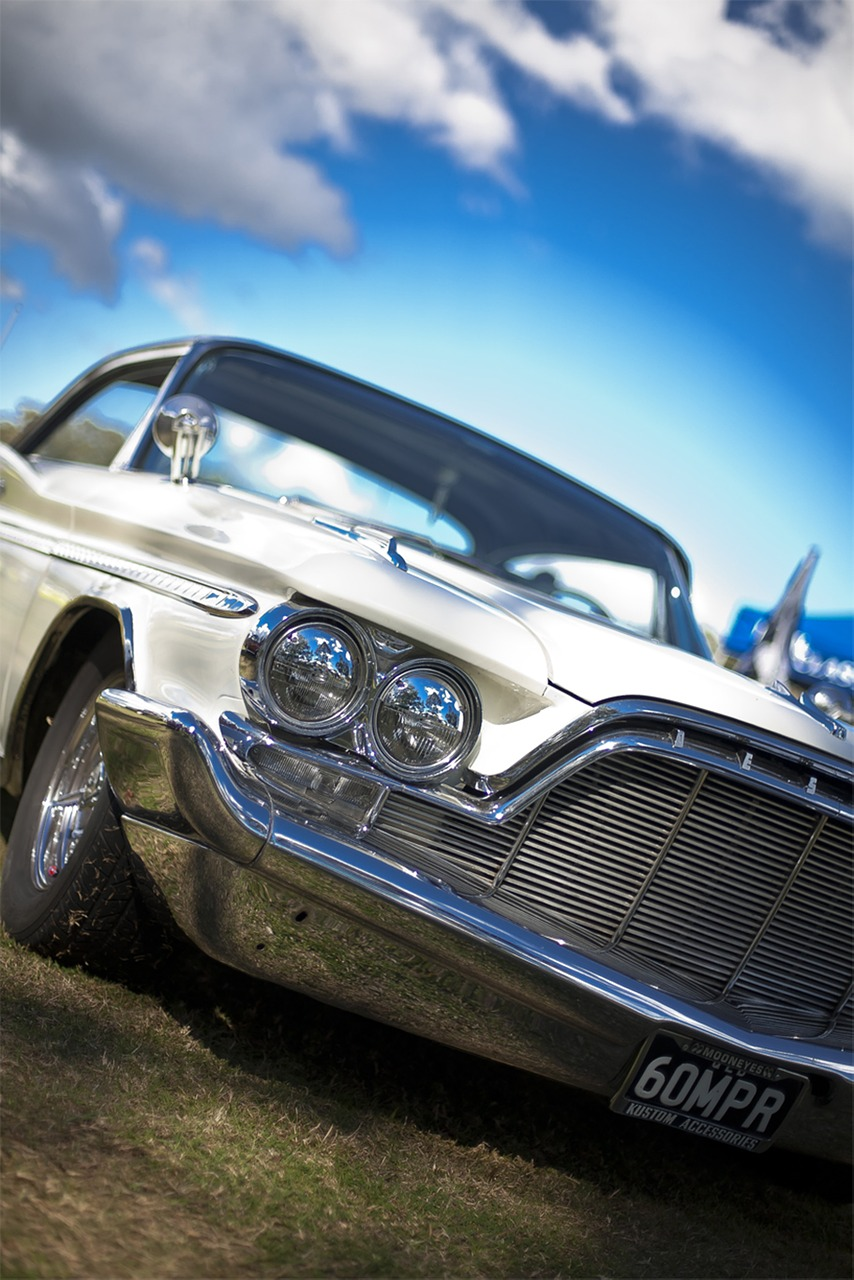
\includegraphics[scale=0.1]{Car1}}
The value of a car dropped from \$7400 to \$6800 over the last year. What percent decrease is this?\\

First, find the absolute change:
\[\$7400 - \$6800 = \$600\]
Then divide this by the \textbf{original amount}:
\[\dfrac{\$600}{\$7400} = 0.081 = 8.1\%\]

Thus, the value of the car dropped by 8.1\%.
\end{example}

\begin{try}[http://izzomath.com/103text/finance/example1.7/story.html]
You go car shopping and find your dream car for \$11,000 sitting on the lot, but unfortunately you only have \$9,000 to pay for it.  You offer the dealership the money you have and they accept your offer.  What percentage did the dealership take off the car?
\end{try}

The base of a percent is very important.  For example, while Nixon was president, it was argued that marijuana is a ``gateway'' drug, using the claim that 80\% of marijuana smokers went on to use harder drugs like cocaine.  The problem is that this isn't true.  The true statistic is that 80\% of harder drug users first smoked marijuana.  The difference is one of base: 80\% of marijuana users versus 80\% of hard drug users.  In reality, out of every 1000 marijuana smokers, about 42 of them go on to use harder drugs, but there are few people who go on to use harder drugs without using marijuana first.

\begin{example}[https://www.youtube.com/watch?v=gB3RqkMzDDE]{Amount Before an Increase}
\marginnote{
\includegraphics[scale=0.08]{Books1}}
If the tuition and fees paid by the average student in the U.S. is \$9,139, and this is 17\% more than the average five years ago, what was the average cost then?\\

The new amount---\$9,139---is 117\% of the original cost:
\[\$9,139 = (117\%)(\textrm{Original Cost})\]
\[\textrm{Original Cost} = \dfrac{\$9,139}{117\%} = \dfrac{\$9,139}{1.17} = \$7,811\]
The original cost, then, was \$7,811 for the average student five years ago.
\end{example}

Relative change or percent differences are also useful when comparing quantities of different sizes, because we can put everything on equal footing to make a meaningful comparison.

\begin{example}[https://www.youtube.com/watch?v=yQmIyPZefK0]{Enrollment Changes}
Generally, more students go to college every semester than the semester before.  In the fall semester of 2008 there were 5,748 students enrolled at Frederick Community College; by the fall of 2009, the number had grown to 6,233.  Compare these two numbers.\\

\marginnote{\bfseries Solution}
We could compare them by simply finding the difference, and saying that there were 485 more students in 2009 than in 2008, but out of context this number is mostly meaningless.  At a small school like FCC, this may represent a dramatic change, but at a larger school like the author's alma mater of North Carolina State, 485 students wouldn't move the needle at all.\\

Instead, we can calculate this as a percentage change:
\[\dfrac{485}{5748} = 0.084 = 8.4\%\]
Enrollment rose by 8.4\%, which is a modest but respectable gain.
\end{example}

\begin{try}[http://izzomath.com/103text/finance/example1.8/story.html]
If you took the SAT twice, scoring 500 on the verbal portion the first time and 620 the second time, by what percentage did your score increase?
\end{try}

This idea of putting different quantities on equal footing in order to compare them is extremely powerful, and crucial in many contexts.  We'll do something similar later when we consider financial applications.  There, we'll be interested in, for instance, comparing two loans with different interest rates and durations and deciding which is more advantageous.  The details will differ, but the concept of finding common ground on which to compare different quantities comes up in many areas.\\

\begin{example}[https://www.youtube.com/watch?v=gSA_go511q4]{Comparisons}
There are 435 Longhorn Steakhouse locations in the U.S. and 136 Ruth's Chris Steakhouse locations.  Compare these two numbers.\\

\marginnote{\bfseries Solution}
Rather than simply saying that there are 299 more Longhorn locations that Ruth's Chris, let's use a meaningful measure like the percentage difference.\\

We could say that Longhorn is \[\frac{299}{136} = 219.9\%\] larger, or that Ruth's Chris is \[\frac{299}{435} = 68.7\%\] smaller.  We could also say that Ruth's Chris is \[\frac{136}{435} = 31.3\%\] of the size of Longhorn.
\end{example}
\text{}\\

The next exercise wraps up the discussion on percentage change by reinforcing the need to be careful with the base of the percent when discussing a change.\\

\begin{example}[https://www.youtube.com/watch?v=SOSt8uYaObc]{A Tricky Percentage Problem}
\marginnote{\includegraphics[scale=0.15]{Taxes1}}
Suppose you originally paid \$1200 in taxes.  A year later taxes decreased by 20\%, but the following year taxes increased by 20\%.  What do you pay in taxes at the end?\\

You may be tempted to jump to the conclusion that you'll pay \$1200 in taxes at the end, since the 20\% decrease was reversed by the 20\% increase.  Be careful, though: the decrease was 20\% of \emph{the original amount} and the increase was 20\% of \emph{the reduced amount}.  Thus, the increase was \emph{smaller} than the increase, so we expect to pay less than \$1200 at the end.\\

Specifically, after one year, the taxes would be $(\$1200)(0.80) = \$960$.  After two years, the taxes would be $(\$960)(1.20) = \$1152$.
\end{example}

\begin{exercises}
\textit{For problems 1--8, convert each number to a percent.}\\
\pfour{$\dfrac{1}{2}$}
\pfour{$0.04$}
\pfour{$\dfrac{3}{5}$}
\pfour{$0.79$}

\pfour{1.35}
\pfour{$\dfrac{10}{4}$}
\pfour{12.5}
\pfour{0.0378}

\textit{For problems 9--16, convert each percent to a decimal.}\\
\pfour{33\%}
\pfour{2.6\%}
\pfour{124\%}
\pfour{1240.5\%}

\pfour{42\%}
\pfour{4.5\%}
\pfour{0.003\%}
\pfour{$\dfrac{1}{4}\%$}

\ptwo{In the fall of 2009 FCC enrolled 6,233 students.  Of those enrolled, 2,810 are in the 18-21 age group.  What percent of FCC students does this represent?}
\ptwo{Patrick left an \$8 tip on a \$50 restaurant bill.  What percent tip is that?}

\ptwo{Ireland has a 23\% VAT (value-added tax, similar to a sales tax).  How much will the VAT be on a purchase of a \euro 250 item?}
\ptwo{Employees in 2012 paid 4.2\% of their gross wages towards social security (FICA tax).  How much would someone earning \$45,000 a year pay toward social security?}

\ptwo{A project on Kickstarter was aiming to raise \$15,000 for a precision coffee press.  They ended up with 714 supporters, raising 557\% of their goal.  How much did they raise?}
\ptwo{Another Kickstarter project for an iPad stylus raised 1,253\% of their goal, finishing with a total of \$313,250 from 7,511 supporters.  What was their original goal?}

\ptwo{One year ago the median price for a home was \$275,000.  Now the current median price for a home is \$235,000.  What was the percent decrease in the median price of a home over the last year?}
\ptwo{There were 943 tornadoes reported in the U.S. in 2013, and 897 tornadoes were reported in 2014.  What percent decrease was there from 2013 to 2014?}

\ptwo{The population of a town increased from 3,250 in 2008 to 4,300 in 2010.  Find the absolute increase and the percent increase.}
\ptwo{The number of CDs sold in 2010 was 114 million, down from 147 million the previous year.  Find the absolute decrease and the percent decrease.}

\ptwo{A company wants to decrease their energy use by 15\%.
\begin{enumerate}[(a)]
\item If their electric bill is currently \$2,200 a month, what will their bill be if they're successful?
\item If their next bill is \$1,700 a month, were they successful?  What percent decrease was there from the current bill?
\end{enumerate}
}
\ptwo{A store is hoping an advertising campaign will increase their number of customers by 30\%.  They currently have about 80 customers per day.
\begin{enumerate}[(a)]
\item How many customers will they have if their campaign is successful?
\item If they increase to 120 customers a day, were they successful?  What percent increase is this from the current level?
\end{enumerate}
}

\ptwo{An article reports that ``attendance dropped 6\% this year, to 300.''  What was the attendance before the drop?}
\ptwo{An article reports that ``sales have grown by 30\% this year, to \$200 million.''  What were sales before the growth?}

\ptwo{The U.S. federal debt at the end of 2001 was \$5.77 trillion, and grew to \$6.20 trillion by the end of 2002. At the end of 2005 it was \$7.91 trillion, and grew to \$8.45 trillion by the end of 2006. Calculate the absolute and relative increase for 2001-2002 and 2005-2006. Which year saw a larger increase in federal debt?}
\ptwo{A TV originally priced at \$799 is on sale for 30\% off. There is then a 9.2\% sales tax. Find the price after including the discount and sales tax.}

\ptwo{The Walden University had 47,456 students in 2010, while Kaplan University had 77,966 students.  Complete the following statements.
\begin{enumerate}[(a)]
\item Kaplan's enrollment was \line(1,0){20} \% larger than Walden's.
\item Walden's enrollment was \line(1,0){20} \% smaller than Kaplan's.
\item Walden's enrollment was \line(1,0){20} \% of Kaplan's.
\end{enumerate}}
\ptwo{In the 2012 Olympics, Usain Bolt ran the 100 m dash in 9.63 seconds.  Jim Hines won the 1968 gold with a time of 9.95 seconds.
\begin{enumerate}[(a)]
\item Bolt's time was \line(1,0){20} \% faster than Hines'.
\item Hines' time was \line(1,0){20} \% slower than Bolt's.
\item Hines' time was \line(1,0){20} \% of Bolt's.
\end{enumerate}}

\ptwo{A store has clearance items that have been marked down by 60\%.  They are having a sale, advertising an additional 30\% off clearance items.  What percent of the original price do you end up paying?}
\ptwo{A publisher marks up a textbook by 65\%, and a bookstore further marks up the textbook by 35\%.  What percentage of the original cost do you pay?}
\end{exercises}
